\documentclass[conference,harvard,brazil,english]{sbatex}
\usepackage[utf8]{inputenc}
\usepackage{ae}
\usepackage{graphicx,url}
\usepackage{graphics}
\usepackage{epstopdf}


\usepackage[brazil]{babel}   
\usepackage[utf8]{inputenc}  
\usepackage{amsmath}

\usepackage{multirow}

\usepackage{subfigure}

\makeatletter
\def\verbatim@font{\normalfont\ttfamily\footnotesize}
\makeatother
\usepackage{amsmath}
% --------------------------------------------------


\begin{document}

% CABEÇALHO

\title{APLICAÇÃO DE REDES SIAMESAS NA AUTENTICAÇÃO DE CONDUTORES}

\author{Andrey Gustavo de Souza}{andrey.souza@estudante.ufla.br}
\address{Departamento de Automática\\ Universidade Federal de Lavras\\ Lavras, Minas Gerais, Brasil}

\author[1]{Wilian Soares Lacerda}{lacerda@dcc.ufla.br}

\author{Carlos H. Q. Forster}{forster@ita.br}
\address{Instituto Tecnológico de Aeronáutica \\ São José dos Campos, SP, Brasil}

\author[1]{Danilo Alves de Lima}{danilo.delima@deg.ufla.br}

\author{Tiago Santana de Nazaré}{tiagosn@usp.br}
\address{Time de \textit{Data Science}, Itaú-Unibanco \\
São Paulo, SP, Brasil}



% \twocolumn apenas para conference
\twocolumn[

\maketitle

\selectlanguage{english}
\begin{abstract}
One of the major limitations of driver authentication and identification systems proposed in the literature is the need to train the models with each new driver to be identified. In this context, this work aims to present the novel application of siamese neural networks (RNS) for driver authentication, exploiting the ability of this network topology to create a feature space that facilitates discriminating drivers, even when such drivers are not in the set of training. With the space created by RNS and distance-based techniques it was possible to discriminate the authenticity of drivers with an AUC higher than 99\%.   \end{abstract}

\keywords{Artificial Neural Networks, Driver Authentication, Siamese Networks, Driver Behavior.}

\selectlanguage{brazil}
\begin{abstract}
 Uma das maiores limitações de  sistemas de autenticação e identificação de condutores propostos na literatura é a necessidade de treinamento dos modelos a cada novo condutor a ser identificado. Sendo assim, este trabalho tem como objetivo apresentar a inédita aplicação de redes neurais siamesas (RNS) para autenticação de condutores, explorando a capacidade que esta topologia para criar um espaço de característica que facilite discriminar condutores, mesmo quando tais condutores não estão no conjunto de treinamento. Com o espaço criado pela RNS e técnicas baseadas em distância foi possível discriminar a autenticidade de condutores com uma AUC superior a 99\%.
\end{abstract}

\keywords{Redes Neurais Artificiais, Autenticação de Condutores, Redes Siamesas, Comportamento de Condutores.}
]

% CONTRIBUIÇÃO

\selectlanguage{brazil}

\section{Introdução}
%Aqui vou dar uma contextualizada sobre o problema endereçado, de modo que se justifique o estudo nesse tema específico
%Falar sobre o problema de roubos e furtos de veículos no Brasil e da necessidade da introdução de opções tecnológicas parar mitigar o problema em questão
%Apresentar a hipótese endereçada pelo trabalho
%aplicações apresentadas de identificação de condutores apresentada por Kar20

Um dos grandes problemas relacionados à segurança pública no Brasil é o número crescente de roubos e furtos de veículos, quando, somente em 2017, foram furtados ou roubados mais de 538 mil veículos em todo país \cite{fbsp2018}. A Figura~\ref{fig:roubos} apresenta a série histórica do número de veículos roubados no Brasil desde 2007, sem considerar furtos, que passaram a ser contabilizados somente a partir de 2013 pelo Fórum Brasileiro de Segurança Pública. Tais números corroboram para a discussão de soluções alternativas e imediatas que visam mitigar este problema, visto que este não só beneficiariam proprietários de veículos, mas também companhias de seguro e forças de segurança pública, que diretamente sofrem com este problema.

\begin{figure}[ht]
\centering
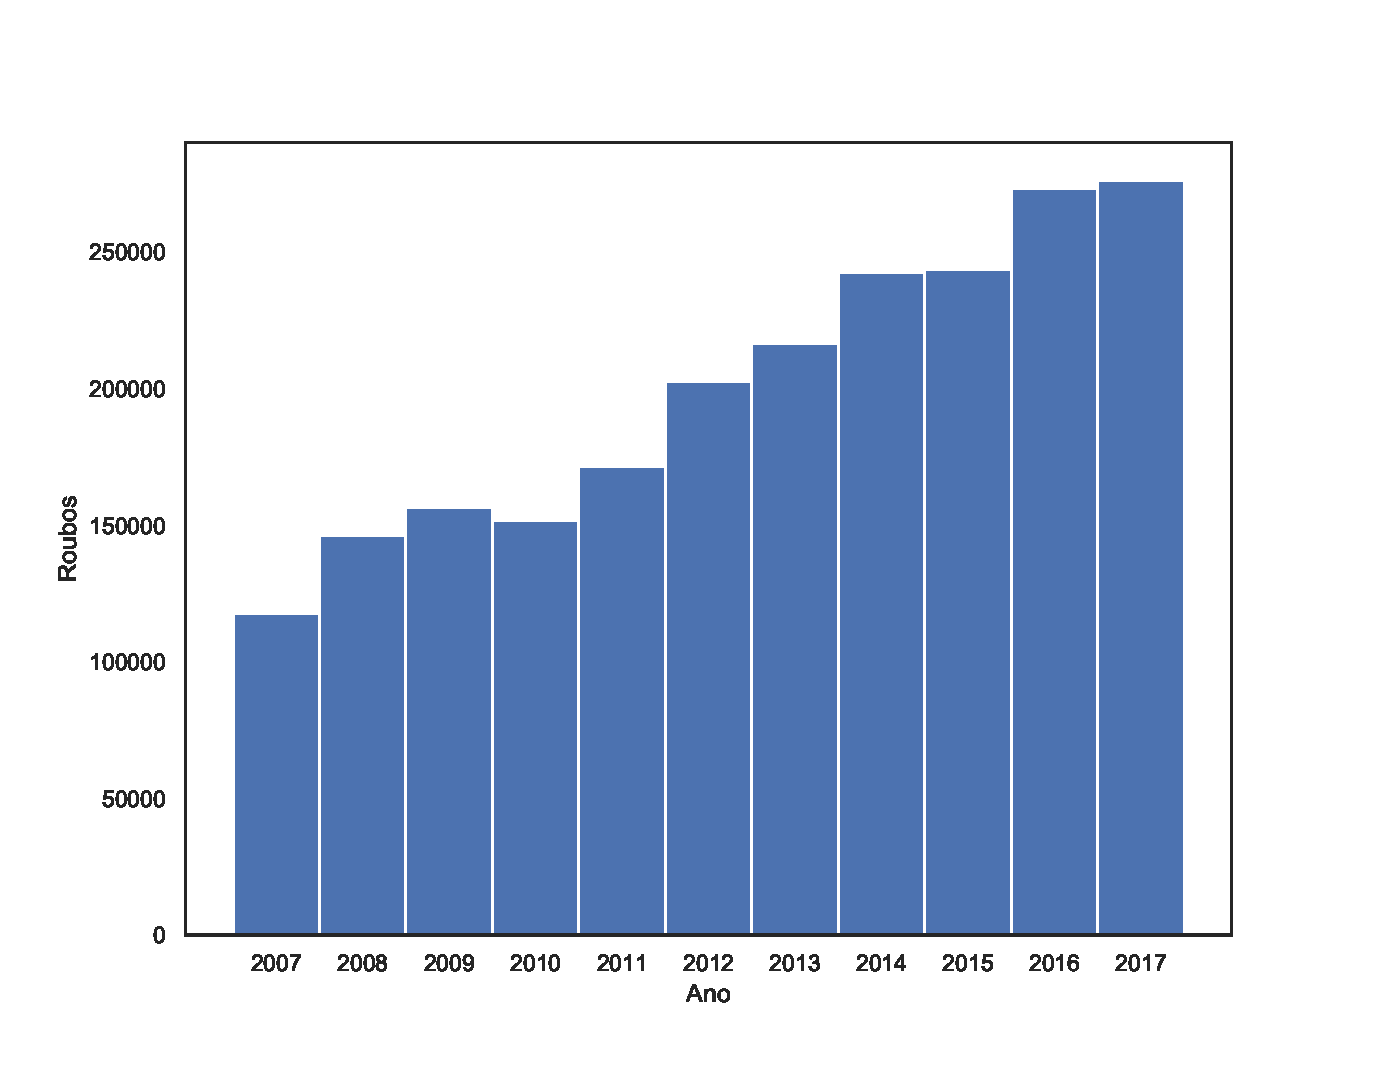
\includegraphics[width=0.46\textwidth]{roubos.eps} \caption{Veículos Roubados no Brasil por ano. Fonte: Adaptado do Fórum Brasileiro de Segurança Pública (2018).}
\label{fig:roubos} 
\end{figure}

Em paralelo a este problema, aplicações envolvendo comportamento de condutores mediante dados de direção têm sido exploradas com diversos objetivos, como detecção de agressividade na direção, sonolência, desatenção, entre outros. Estas aplicações envolvendo comportamento do condutor também podem ser aplicadas para a autenticação e/ou identificação destes condutores em um determinado veículo. Isto é possível devido ao estilo de direção único que cada condutor tem e que podem ser identificados por meio da aplicação de técnicas de aprendizado de máquina. Na literatura, autenticação e identificação têm sido objeto recente de estudo e têm ganhado interesse não só de acadêmicos, mas também de fabricantes de veículos estimulados pelo impacto que aplicação de tais funcionalidades teriam no mercado automotivo.

Porém o estado da arte desta temática ainda passa por diversas limitações que impedem a implementação real deste tipo de sistema. Entre estas limitações, podem-se destacar a necessidade que algoritmos de aprendizado de máquina têm de serem retreinados a cada novo condutor introduzido no modelo de identificação ou autenticação de um veículo ~\cite{Wang2017a,Burton2017,Martinez2016a,Ezzini2018}. Diante de tal cenário, este trabalho tem como objetivo estudar alternativas para a autenticação de condutores que não demandem novo treinamento a cada novo condutor ou veículo em que o modelo venha a ser aplicado.

Tara tal é feita a aplicação de Redes Neurais Siamesas, uma topologia de Redes Neurais Artificiais, desenvolvida para determinar se pares de entradas de dados são ou não da mesma classe, como identificação facial ou de assinaturas em imagens. Estas redes realizam em cada uma das entradas uma transformação que visa aproximar espacialmente dados de uma mesma classe e afasta dados classes diferentes. Logo, esta rede pode ser usada para a indicação se uma amostra de sensores do veículo de um condutor pertence a um conjunto de dados de um grupo de condutores autorizados. Tal abordagem, até então, é inédita.

Este trabalho está dividido da seguinte forma: a seção~\ref{sec:trab_rel} apresenta o estado da arte referente à detecção de comportamento de condutores, bem como a temática de autenticação e identificação de condutores. Por sua vez a seção~\ref{sec:siamese} traz uma introdução às Redes Neurais Siamesas, assim como seu funcionamento e formulação. Os materiais e métodos usados nos experimentos são apresentados na seção~\ref{sec:met}, enquanto os resultados são denotados em seguida na seção~\ref{sec:results}, juntamente com discussões sobre os mesmos. Por fim, conclusões e considerações finais são apresentados na seção~\ref{sec:finais}.


\section{Trabalhos Relacionados} \label{sec:trab_rel}

Dados provenientes do barramento de comunicação \textit{Controller Area Network} (CAN-bus) do veículo trazem em si informações relevantes sobre a dinâmica de direção do veículo. Estes dados podem ser utilizados na detecção e modelagem de certos padrões e comportamentos de direção do condutor tais como agressividade, sonolência, fadiga, distração, embriaguez, entre outros \cite{Meiring2015}. Outra fonte de informações referentes à dinâmica de direção são os sensores inerciais (IMU), que vêm embarcados em \textit{smartphones} e dispositivos dedicados a esta função que, utilizados em conjunto com os dados do CAN-bus, podem potencializar a detecção dos comportamentos do condutor supracitados \cite{Kaplan2015}.


%falar agora da identificação de condutores. Iniciar falando do trabalhos do Wakida por ser o primeiro registro desta aplicação (pelo menos a encontrada). Depois falar sobre DelCampo2014, por usar análise cepstral e RNAs. 
%trazer uma definição do que é autenticação e identificação de condutores
Dente estas aplicações do uso deste dados é a autenticação e identificação de condutores. Autenticação de condutores é a funcionalidade que um sistema tem em definir se um determinado condutor pertence ao grupo de condutores autorizados a operar o veículo. Por sua vez, identificação de condutores é definida como a funcionalidade que um sistema tem de identificar um condutor específico entre um grupo de condutores que estão aptos a operar um determinado veículo. 

Trabalhos recentes exploram outros panoramas relacionados à identificação e autenticação de condutores. \citeasnoun{jafarnejad2017} explora o impacto no número de condutores do desempenho dos modelos de identificação, mostrando que quanto maior a população de condutores conhecidos pelo modelo, menor a capacidade deste discernir entre os condutores. Um modelo baseado em pré-processamento dos dados e o algoritmo \textit{Extra-Trees} formado por etapas de autenticação e subsequente identificação foi implementado por \cite{sbrc}, com objetivo de identificar intrusos e também gerar configurações personalizadas de funções veículo para cada usuário identificado. Este trabalho também utiliza sensores virtuais, como forma de contornar a situação onde veículos pouco sofisticados são providos de menos sensores.

%agora introduzir a contribuição do trabalho para o tema, bem como as novidades que não foram aplicadas à outros trabalhos

Contudo, todos os trabalhos supracitados têm um fator limitante para aplicações práticas de um sistema de autenticação/identificação de condutores: a necessidade de treinamento do modelo a cada novo condutor que possa a vir conduzir o veículo. Tem-se o fato de que o poder de processamento das centrais do veículo é limitado, o que poderia demandar da implementação de um hardware mais robusto, que elevaria os custos de tal sistema. Sendo assim, este trabalho propõe o uso de um modelo pré-treinado que não necessita de posterior treinamento mesmo em casos onde o novo condutor é desconhecido pelo modelo. Este modelo é feito por meio do uso de Redes Neurais Siamesas, conhecidas por sua aplicação em reconhecimento facial e em casos onde o número de dados por indivíduo é limitado. Na seção a seguir, é apresentada uma breve introdução à este tipo de Rede Neural Artificial (RNA), onde é demonstrado seu princípio de funcionamento e como ela pode ser aplicada no problema de identificação de condutores.

\section{Redes Neurais Siamesas} \label{sec:siamese}
%Falar sobre aprendizado por similaridade, e como este conceito está relacionado com o problema de identificação de condutores;
%Introduzir o conceito de redes siamesas, como aplicações originais, seu potencial para reconhecimento facial e de objetos; 
    %Colocar figura ilustrativa que mostra seus elementos;
    %Falar da contrastive loss e do uso de medidas de distância no treinamento da rede;
    %O que fazer com a rede após esta é treinada?
    
Redes Neurais Siamesas (RNS) foram introduzidas por \cite{bromley1994}, onde foram utilizadas para realizar a verificação de assinaturas. A arquitetura de uma RNS, tal qual mostrado na Figura~\ref{fig:siamese}, consiste em duas redes neurais que compartilham de pesos idênticos que são ligadas por uma ou mais camadas. Na maioria dos casos, uma RNS executa uma codificação não linear dos dados de entrada com o objetivo de atingir um espaço semanticamente significativo onde padrões relacionados sejam próximos uns dos outros (tais como faces de pessoas, assinaturas, entre outros) e os não relacionados sejam distantes uns dos dos outros \cite{Harandi}.

\begin{figure}[ht]
\centering
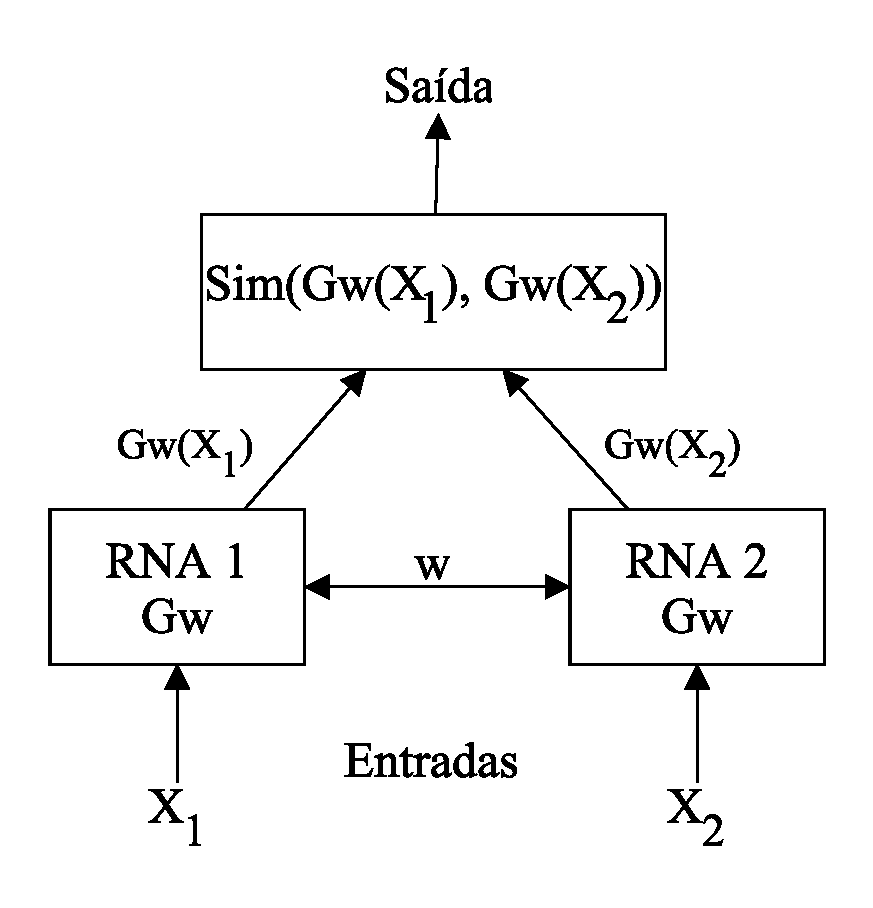
\includegraphics[width=.35\textwidth]{im1.eps}
\caption{Arquitetura de uma Rede Neural Siamesa.}
\label{fig:siamese}
\end{figure}

Uma RNS recebe como entrada um par de leituras, tanto no treinamento quanto no teste, com o objetivo de desenvolver similaridade entres pares de uma mesma classe $Y$, a classe genuína e a distanciar pares de dados de classes diferentes a classe impostora. A partir do treinamento a rede cria um espaço multi-dimensional $G_w(X)$ igual ao número de neurônios de saída da rede neural base, rede esta que é compartilhada entre os pares de entrada. A representação espacial de cada entrada então é submetida à uma função de similaridade $Sim(G_w(X_1), G_w(X_2))$, normalmente sendo uma medida de distância Euclidiana. A função  similaridade baseada na medida de distância Euclidiana é obtida da seguinte forma:

\begin{equation}
\resizebox{.85\hsize}{!}{$Sim(G_w(X_1), G_w(X_2)) =  \sqrt{[G_w(X_1) - G_w(X_2)]^2}$}
\end{equation}

\noindent onde $G_w(X_1)$ e $G_w(X_1)$ são dois pontos no espaço multidimensional criado pelos parâmetros compartilhados $w$ quando mapeiam as entradas $X_1$ e $X_2$.

Uma vez obtida a medida de similaridade, é definido se os dados de entrada pertencem ou não à uma mesma classe dado um limiar de distância definido. Como função de perda (\textit{loss function}), RNS fazem uso da Perda Contrastiva (\textit{Contrastive Loss)} para o treinamento. Esta função perda, introduzida por \cite{Chopra2005}, é calculada através do somatório das perdas individuais para pares genuínos e impostores. Quando pares genuínos estão muito distantes, estes são penalizados por $L_G$. Por sua vez, pares impostores que estão dentro valor limiar de distância, são penalizados por $L_I$. As redes irmãs têm seus pesos atualizados via \textit{backpropagation}. Então a cada época de treinamento, pares genuínos são atraídos a um sub-espaço próximo, enquanto pares impostores são mantidos a uma distância acima da margem definida. A função de perda contrastiva é definida da seguinte forma:

\begin{equation*}
    L_G = (1 - Y_A)Y_p^2\\
\end{equation*}
\begin{equation}
    L_I  = Y_A(max(M-Y_P,0))^2
\end{equation}
\begin{equation*}
    L =L_G + L_I,
\end{equation*}

\noindent onde $Y_A$ e $Y_P$ são valores binários que são iguais a 1 para pares genuínos e 0 para impostores. $Y_A$ e $Y_P$ são, respectivamente, o valor real dos pares e o retornado pela RNS. $M$ é o valor de margem da distância que define quais pares são genuínos ou impostores \cite{Martin2017}.

%falar sobre como as redes siamesas podem ser usadas para aprender features de um conjunto de dados: https://sorenbouma.github.io/blog/oneshot/ - falar sobre one-shot learning

   
\section{Materiais e Métodos}\label{sec:met}
%Esse nome pode (ou deve) mudar para algo mais "rebuscado". Descrever que nesta seção serão apresentados os insumos utilizados tal qual os procedimentos adotados para o desenvolvimento do modelo;

Nesta seção serão apresentados os insumos utilizados para o desenvolvimento do modelo de autenticação de condutores, tal como o \textit{dataset} utilizado e sua descrição e também qual foi a metodologia adotada na implementação de tal modelo. 

\subsection{O \textit{Dataset}}
%Dar detalhes sobre o dataset utilizado; qual o dataset? de onde ele vem? qual o tamanho, numero de classes, contexto no qual os dados foram coletados? Quais a vantagem de se usar esse dataset para o desenvolvimento do modelo em questão?

Para a implementação deste trabalho, foi utilizado o \textit{Driving Behavior Dataset} disponibilizado pelo \textit{Laboratory of Advanced Collaboration} da PUC Rio. Estes dados foram coletados por \cite{OLIVEIRAVASCONCELOS2017a} para a detecção de anomalias durante a condução do veículo. Estes dados foram obtidos pela leitura do CAN-bus do veículo através da porta OBD-II do mesmo, em comunicação com um \textit{smartphone} que também fornece dados oriundos de unidade de medidas inerciais e de geolocalização embarcados no dispositivo. 

Cada um dos vinte e cinco motoristas voluntários percorreu um mesmo trajeto de 14.5 km entre as 09:00 e 20:00 em dias úteis. Os motoristas diferem entre si quanto a experiência como motorista (2 à 42 anos), idade (20 a 60 anos) e gênero (dezesseis do sexo masculino e nove do sexo feminino). O \textit{dataset} contém no total 12.5 horas de condução com um percurso total de 362.5 km. 

\subsection{Tratamento prévio dos dados}
%Mostrar os passos que foram dados para se chegar no modelo final;
    %Filtragem dos dados (médias móveis) e explicar porque a janela temporal foi escolhida (ter tempo suficiente para a velocidade sair do zero), quanto maior o tempo, melhor a extração de características (citar artigo cba)
    
    %Divisão entre treinamento e teste (explicar que alguns condutores serão usados para a criação do modelo da rede siamesa e outros serão usados para a validação do mesmo

Antes de serem utilizadas na implementação e teste do modelo, os dados passam por um pré-processamento com o objetivo de se eliminar ruídos nas leituras. O método utilizado foi o da médias móveis, que consiste na extração das médias em janelas deslizantes com tamanho definido. As médias móveis são obtidas para cada trajeto de cada condutor. A janela definida foi de 90 segundo, janela esta que maximiza a extração de características de cada condutor \cite{DeSouza2018}.

Após esta etapa, os dados são divididos aleatoriamente em treinamento e teste. Esta divisão é feita considerando um grupo de condutores cujos dados serão utilizados para o treinamento da RNS e o restante serão utilizados para validação do modelo. A proporção usada em treinamento e teste foi de 50\%, com o objetivo de se garantir o maior número de testes de desempenho do modelo de autenticação de condutores. A Tabela~\ref{tab:div} apresenta quais condutores foram selecionados para treinamento e teste do modelo.

\begin{table}[ht]
\caption{Divisão dos condutores em treinamento e teste.}
\centering
\begin{tabular}{|l|l|}
\hline
\multicolumn{1}{|c|}{Grupo} & \multicolumn{1}{c|}{Condutores} \\ \hline
Treinamento & \begin{tabular}[c]{@{}l@{}}8, 16, 0, 23, 11, 9, 13, \\ 1, 22, 5, 2, 12, 15\end{tabular} \\ \hline
Teste & \begin{tabular}[c]{@{}l@{}}3, 4, 6, 7, 10, 14, 17, \\ 18, 19, 20, 21, 24\end{tabular} \\ \hline
\end{tabular}
\label{tab:div}
\end{table}

Os doze condutores selecionados para teste são divididos em quatro grupos, simulando condutores que utilizam um mesmo veículo. São efetuados para cada veículo testes, onde os condutores de cada um destes são confrontados com condutores de outros veículos, que serão para o veículo em questão impostores. A Tabela~\ref{tab:veic} apresenta como os condutores estão divididos em veículos.

\begin{table}[ht]
\caption{Divisão dos condutores de teste em veículos.}
\centering
\begin{tabular}{|c|l|}
\hline
\textbf{Veículo} & \multicolumn{1}{c|}{\textbf{Condutores}} \\ \hline
1 & 3, 4, 6 \\ \hline
2 & 7, 10, 14 \\ \hline
3 & 17, 18, 19 \\ \hline
4 & 20, 21, 24 \\ \hline
\end{tabular}
\label{tab:veic}
\end{table}

Os dados antes de utilizados no treinamento da RNS são submetidos a um reescalamento de seus valores entre 0 e 1. Este passo é importante, visto que os dados tem magnitudes de valores diferentes, o que é prejudicial para o treinamento de uma RNA, onde esta pode dar mais importância a variáveis cujos valores tem maior amplitude. É importante ressaltar que o valor mínimo e máximo usados para transformar o conjunto de treinamento são os mesmo usados para o conjunto de teste. 

% \begin{figure}[!ht]
% \centering
% \includegraphics[width=1\textwidth]{sliding.eps}
% \caption{Janela deslizante.}
% \label{fig:corr}
% \end{figure}


\subsection{Desenvolvimento do Modelo}
%Apresentar a topologia da rede siamesa que será utilizada; destacar a quantidade de camadas, qual o algoritmo de treinamento (otimizador) bem como quais os hiper-parâmetros que deverão ser ajustados;

A implementação do modelo de autenticação de condutores passa por duas etapas. A primeira destas é construção e treinamento da Rede Neural Siamesa, de modo a garantir um modelo de representação espacial dos dados de entrada que consiga descrever bem as características de condução de cada condutor. A segunda etapa consiste em fazer uso do modelo base da RNS implementada na primeira etapa para criar para cada veículo um suporte de dados derivados a partir de dados de cada condutor autorizado. A função de decisão é baseada no algoritmo não supervisionado de NN, com base numa distância limiar, ou seja, se $D>T$ então não autorizado, senão, autorizado.

Para a implementação da RNS, primeiro são formados pares entre leituras dos dados em pares genuínos (classe 1) e pares impostores (classe 0), com respeito à identidade dos condutores alocados na base de treinamento. A proporção entre as classes foi de 50\% e também garantindo que se tenham pares impostores formados por todas as combinações de condutores da bases. Para o teste de desempenho da RNS, pares também são formados por condutores da base de teste. O próximo passo é definir a topologia do modelo base da RNS. O modelo base é uma rede neural que é configurada de acordo com os tipos de dados de entrada, sendo geralmente um modelo sequencial, baseado em camadas convolucionais (para imagens), recorrentes como a LSTM (processamento de linguagem natural) ou em perceptron de múltiplas camadas (MLP) para dados estruturados, sendo este último a base do modelo implementado neste trabalho.

O modelo base é composto por um número variável de camadas (duas e três) e o número de neurônios em cada uma destas camadas é um hiper-parâmetro que é avaliado durante os testes de desempenho dos modelos. A ativação usada na saída de cada um dos neurônios é a \textit{Leaky ReLu}, que, diferentemente da ReLu, não zera saídas negativas dos neurônios, o coeficiente angular para ativações negativas foi fixado em 0.3. Uma camada \textit{Dropout} de 10\% é adicionada nas camada densas intermediárias. Antes das saídas do modelo base serem submetidas à perda contrastiva, estas são submetidas à uma normalização L2 (Euclidiana) para que a distância entre as características geradas sejam normalizadas e tal que a margem de distância entre classes possa ser constante e independente da escala da saída da rede base \cite{SchroffKP15}. A Figura~\ref{fig:base} mostra a topologia da RNS desde a entrada até a saída que será submetida à função de similaridade.

\begin{figure}[!ht]
\centering
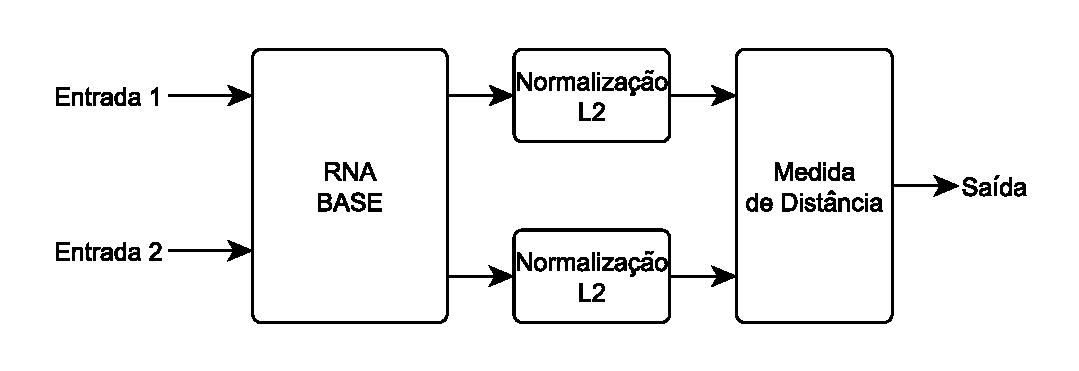
\includegraphics[width=0.47\textwidth]{base.eps}
\caption{Configuração do modelo RNS.}
\label{fig:base}
\end{figure}

São testados três topologias diferentes para o modelo base. A primeira é uma RNA simples com duas camadas de 16 e 8 neurônios respectivamente (RNS 1). A segunda rede é uma RNA com um número maior de neurônios por camada (32 e 16), de modo a se comparar o impacto deste incremento no desempenho da RNS (RNS 2). A terceira topologia é uma RNA de três camadas com 32, 16 e 8 neurônios em cada uma destas camadas (RNS 3). É válido ressaltar que a dimensão do espaço de representação é a quantidade de neurônios da camada de saída do modelo base da RNS. Outros hiperparâmetros devem ser definidos para a implementação da RNS, como a margem de distância $M$, fixada em 0.2. Para o treinamento desta rede foi considerado o algoritmo de otimização RMSprop \cite{hinton2012neural}, com taxa de aprendizado de 0.001, 40 épocas de treinamento, \textit{batch size} de 64 e acurácia como métrica de treinamento.

A hipótese central deste trabalho é o uso de uma RNA que possa mapear características de um mesmo condutor em um sub-espaço próximo, mesmo que dados referentes à direção deste condutor não sejam usados para o treinamento desta rede. Para tanto, é utilizado o modelo base da RNS treinado como extratora de características e dados de novos condutores são submetidos à esta rede. Então, um suporte de dados derivados de cada novo condutor é criado. Partindo do pressuposto que o modelo base tende a aproximar as saídas de dados um mesmo condutor, a formação deste suporte permite que novas leituras dos sensores sejam aplicadas neste modelo e comparadas com os dados salvos. Se os dados submetidos tiverem uma distância próxima das de algum condutor autorizado existe uma alta probabilidade deste condutor ser genuíno. Em contrapartida, se uma leitura dos sensores de algum condutor for distante dos dados de suporte existe chance desse condutor ser um impostor.

Para a execução destes testes, os condutores do grupo de teste são divididos em quatro veículos com três condutores autorizados em cada um destes, tal qual mostrado na Tabela~\ref{tab:veic}. Então, os dados são submetidos ao modelo base e sua saída será utilizada para a tarefa de autenticação de condutores. Para tal, foi efetuada um divisão dos dados derivados de cada condutor para a formação do conjunto de treinamento (40\%) e para testes de autenticidade (60\%). 

A função de decisão que determinará a autenticidade de um condutor em um veículo será baseada na menor distância entre o ponto testado e um outro ponto pertencente ao suporte. Se esta distância for menor que um limiar determinado, o condutor é considerado autêntico e em caso contrário impostor. Considerando $x_i$ uma leitura de um condutor que se deseja autenticar e $X_S$ o suporte de dados do conjunto de condutores autorizados $S$ temos a seguinte função de decisão booleana $F(x_i)$:

\begin{equation}
    F(x_i) = \min_{X_S \in S}(D(x_i,X_S)) < T,
\end{equation}

\noindent onde $D$ é a medida de distância do ponto testado para todos dos pontos do suporte, neste caso Euclidiana e $T$ é o limiar de distância. 

Para medir o quanto o modelo consegue distinguir entre condutores autênticos e impostores, será usado a AUC-ROC. AUC (\textit{Area Under the Curve}) é a área abaixo da curva Característica de Operação do Receptor ROC (\textit{Receiver Operating Characteristics}). Enquanto a ROC é uma curva de probabilidade, a AUC é uma medida de separabilidade entre classes. Uma AUC próximo de 1 indica que o modelo consegue separar bem as classes e próximo de 0.5 indica que o modelo não tem capacidade discriminativa de distinguir entre as classes positivas e negativas. Uma AUC próxima de 0 indica que o modelo está comutando entre classes ou seja, predizendo a classe negativa como positiva e vice-versa. Um vantagem de se usar a AUC-ROC neste caso é a funcionalidade de determinação do limiar (\textit{threshold}) que realiza a separação entre classes autêntico e impostor. É possivel determinar o limiar observando o \textit{trade-off} entre a taxa de falsos positivos e verdadeiros positivos.

\section{Resultados e Discussões}\label{sec:results}
%Comentar sobre os resultados, e como eles estarão divididos em duas partes: 
%Primeiro falar sobre o treinamento da rede siamesa, e qual a acurácia para amostras out-of-sample
%Apresentar também como os dados se comportam depois de passados pelo modelo

A primeira parte da implementação do modelo de autenticação de condutores é o treinamento das RNS especificadas de maneira a determinar a topologia adequada para a tarefa de autenticação de condutores. Como nesta etapa o problema trata de um problema de classificação binário, determinar se o par de entradas corresponde à mesma pessoa ou não, a métrica avaliada é a acurácia. A Figura~\ref{fig:acc} apresenta a acurácia média para a base de teste, onde observa-se que a RNS 2 obteve uma acurácia média maior, bem como menor desvio da mesma, o que indica que esta topologia é a mais adequada para realizar o mapeamento das características dos dados de direção de cada condutor. As RNS 1 e 3 obtiveram maiores desvios de valores da acurácia e desempenho inferior se comparadas à RNS 2. Para a RNS 1, isto pode ser explicado pelo menor número de neurônios desta rede, o que pode reduzir a capacidade da mesma em mapear as características de cada condutor. Por sua vez, o maior número de neurônios da RNS 3 acarreta em um maior número de parâmetros a serem ajustados, o que provoca maior dificuldade de otimização dos pesos da rede com relação às características dos condutores. 

\begin{figure}[!ht]
\centering
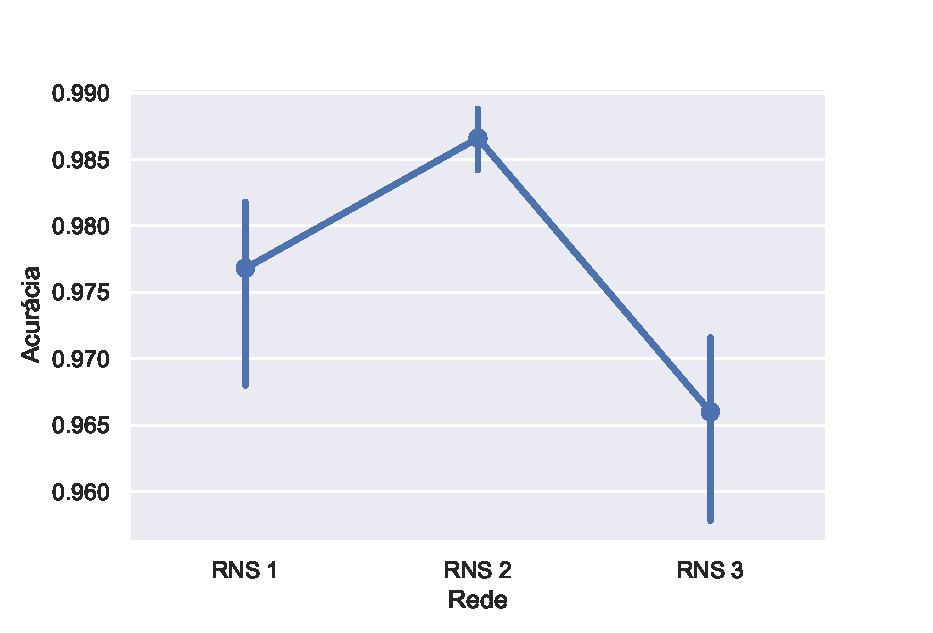
\includegraphics[width=.45\textwidth]{acc.eps}
\caption{Acurácia média obtida em cada uma das topologias da RNS.}
\label{fig:acc}
\end{figure}

Uma vez de posse da rede base que compõe a RNS treinda, é feita a transformação dos dados de direção dos condutores de teste. Como a dimensão dos dados derivados é a quantidade de neurônios da camada de saída da rede base, foi aplicado Análise de Componentes Principais (PCA) para a visualização dos dados. A Figura~\ref{fig:pca} apresenta o conjunto de dados de suporte para o os condutores do veículo 1 obtidos através da rede base da RNS 2. Pode-se constatar que os dados de cada condutor são aglomerados em regiões próximas no espaço de representação, o que indica a viabilidade do uso destes dados para técnicas de autenticação de condutores baseado similaridade espacial, tal como a distância euclidiana.

\begin{figure}[!ht]
\centering
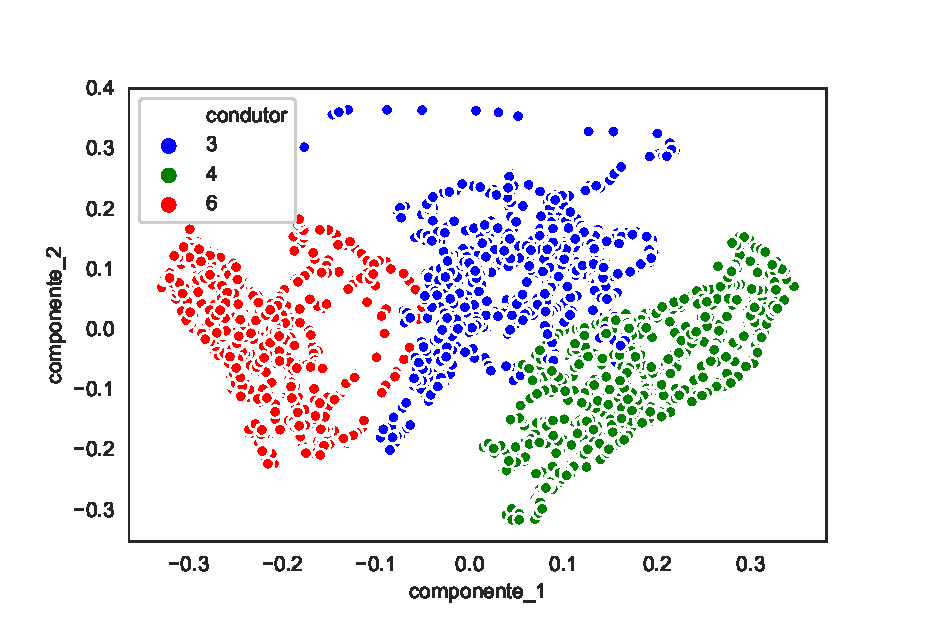
\includegraphics[width=0.45\textwidth]{pca.eps}
\caption{PCA com dois componentes dos dados de suporte gerados pela RNS 2 para o Veículo 1.}
\label{fig:pca}
\end{figure}

Outra forma de determinar se o espaço criado pela rede base agrupa os dados de cada condutor em regiões próximas é a aplicação do algoritmo de clusterização k-\textit{means} em conjunto com a métrica de largura de silhueta (\textit{Silhouette Score}). A maior largura de silhueta em um conjunto de clusters testados no k-\textit{means} indica que este número de clusters é o ideal. Aplicando o k-\textit{means} no espaço criado, observou-se que a quantidade de clusters ideal é 12, tal qual mostrado pela Figura~\ref{fig:kmeans}, igual ao número de condutores de teste. Esta análise indica que o espaço gerado pela rede base consegue aglomerar bem dados de um mesmo condutor e separa aqueles que pertencem à condutores distintos.

\begin{figure}[!ht]
\centering
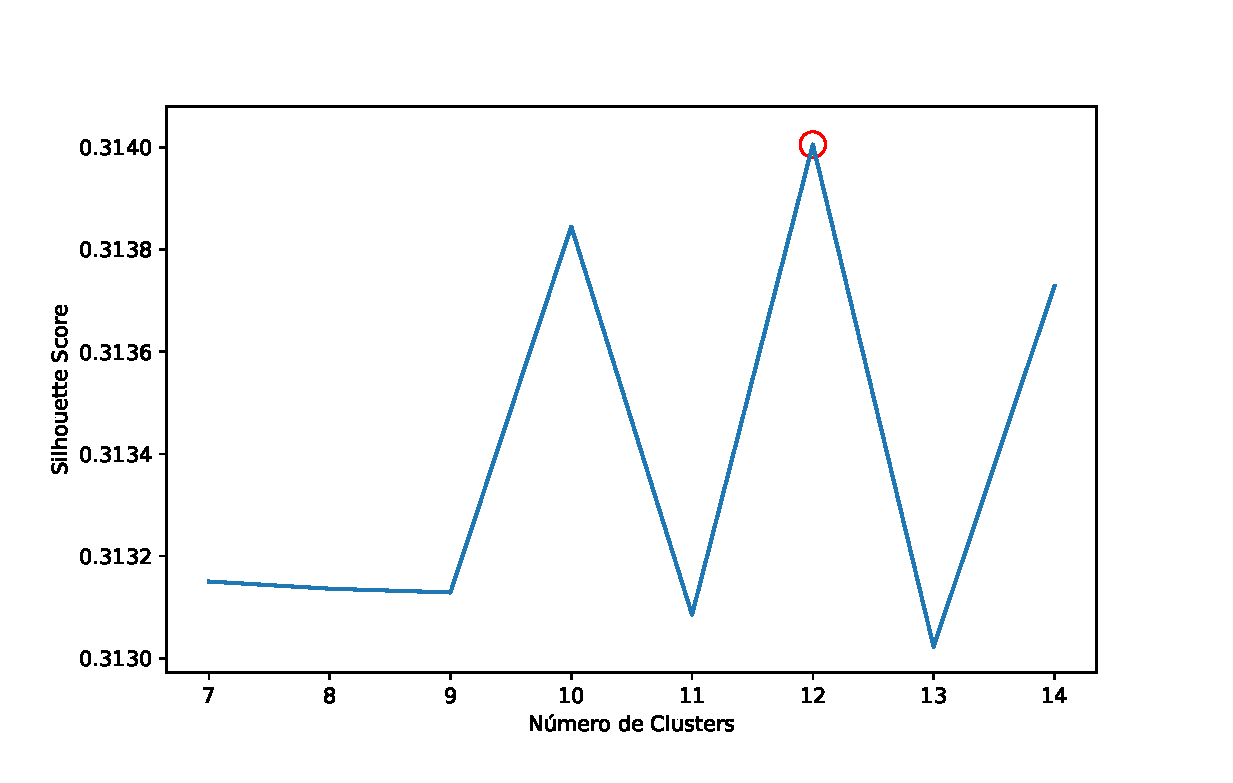
\includegraphics[width=0.45\textwidth]{kmeans.eps}
\caption{Gráfico de silhueta para o algoritmo de agrupamento k-\textit{means} para diversos números de clusters.}
\label{fig:kmeans}
\end{figure}

Para a etapa de autenticação de condutores foram testados também todas as topologias de RNS implementadas, uma vez que não se têm garantias que a acurácia obtida na RNS para autenticação de pares é correlacionada ao desempenho da função de decisão. Para cada RNS treinada é formado um conjunto de suporte dos dados de condução dos condutores de cada veículo, tanto para treinamento quanto para validação. Com os dados de treinamento é inferido um modelo de Vizinho mais Próximo (\textit{Nearst Neighbour} - NN) que quando uma nova leitura é submetida a este, é retornado a distância do ponto mais próximo do conjunto de treinamento. O conjunto de teste é composto por amostras autênticas do veículo testado e amostras de teste de condutores de outros veículos que são considerados impostores. Os veículos são testados em pares de forma a se mensurar a capacidade do modelo NN de separar corretamento condutores, que é medido através da AUC-ROC. 

As Tabelas~\ref{tab:aucteste1},~\ref{tab:aucteste2},~\ref{tab:aucteste3} mostram a AUC média de cada par de veículos em cada um das topologias RNS testadas. Observa-se que desempenho do modelo NN é atrelado também ao desempenho da RNS, onde a RNS 2 têm desempenho ligeiramente superior às outras duas topologias testadas. Outro ponto é que existe uma confusão maior da determinação da autenticidade de condutores em determinados pares de veículos, como quando condutores do veículo 1 são testados no modelo do veículo 3 e vice-versa. Este problema pode ser resultado da semelhança do estilo de direção entre condutores. Contudo, mesmo nesses casos a AUC-ROC obtida é adequada, onde o mínimo obtido foi de 0.949. A Figura~\ref{fig:roc} apresenta a curva ROC para cada um dos veículos analisados quando confrontados com condutores de outros veículos para a RNS 2, que obteve obteve o melhor desempenho geral para a tarefa de autenticação de condutores. As curvas apresentadas indicam uma boa relação entre as taxas de verdadeiros positivos e falsos positivos, o que aponta a viabilidade do uso de RNS para a tarefa de autenticação de condutores.

\begin{table}[!ht]
\caption{AUC-ROC média para condutores autênticos contra condutores de outros veículos (impostores) para a RNS 1.}
\centering
\resizebox{1\columnwidth}{!}{
\label{tab:aucteste1}
\begin{tabular}{|c|c|c|c|c|}
\hline
\multirow{2}{*}{Veículo} & \multicolumn{4}{c|}{Condutores Impostores} \\ \cline{2-5}  
 & 1 & 2 & 3 & 4 \\ \hline
1 & - & 0.989$\pm$0.011 & 0.958$\pm$0.008 & 0.987$\pm$0.008 \\ \hline
2 & 0.990$\pm$0.009 & - & 0.984$\pm$0.008 & 0.998$\pm$0.002 \\ \hline
3 & 0.971$\pm$0.012 & 0.986$\pm$0.011 & - & 0.988$\pm$0.007 \\ \hline
4 & 0.987$\pm$0.005 & 0.996$\pm$0.001 & 0.983$\pm$0.005 & - \\ \hline
\end{tabular}}
\end{table}

\begin{table}[!ht]
\caption{AUC-ROC média para condutores autênticos contra condutores de outros veículos (impostores) para a RNS 2.}
\centering
\label{tab:aucteste2}
\resizebox{1\columnwidth}{!}{
\begin{tabular}{|c|c|c|c|c|}
\hline
\multirow{2}{*}{Veículo} & \multicolumn{4}{c|}{Condutores Impostores} \\ \cline{2-5}  
 & 1 & 2 & 3 & 4 \\ \hline
1 & - & 0.988$\pm$0.006 & 0.972$\pm$0.014 & 0.989$\pm$0.007 \\ \hline
2 & 0.978$\pm$0.007 & - & 0.984$\pm$0.012 & 0.997$\pm$0.001 \\ \hline
3 & 0.949$\pm$0.025 & 0.980$\pm$0.012 & - & 0.984$\pm$0.005 \\ \hline
4 & 0.991$\pm$0.003 & 0.999$\pm$0.001 & 0.991$\pm$0.006 & - \\ \hline
\end{tabular}}
\end{table}

\begin{table}[!ht]
\caption{AUC-ROC média para condutores autênticos contra condutores de outros veículos (impostores) para a RNS 3.}
\centering
\label{tab:aucteste3}
\resizebox{1\columnwidth}{!}{
\begin{tabular}{|c|c|c|c|c|}
\hline
\multirow{2}{*}{Veículo} & \multicolumn{4}{c|}{Condutores Impostores} \\ \cline{2-5} 
 & 1 & 2 & 3 & 4 \\ \hline
1 & - & 0.978$\pm$0.006 & 0.949$\pm$0.014 & 0.991$\pm$0.007 \\ \hline
2 & 0.988$\pm$0.070 & - & 0.980$\pm$0.012 & 0.999$\pm$0.001 \\ \hline
3 & 0.972$\pm$0.025 & 0.984$\pm$0.012 & - & 0.991$\pm$0.005 \\ \hline
4 & 0.989$\pm$0.003 & 0.997$\pm$0.001 & 0.984$\pm$0.006 & - \\ \hline
\end{tabular}}
\end{table}

\begin{figure*}[!ht]
\makebox[\linewidth][c]{
    \centering
    \subfigure[Veículo 1]{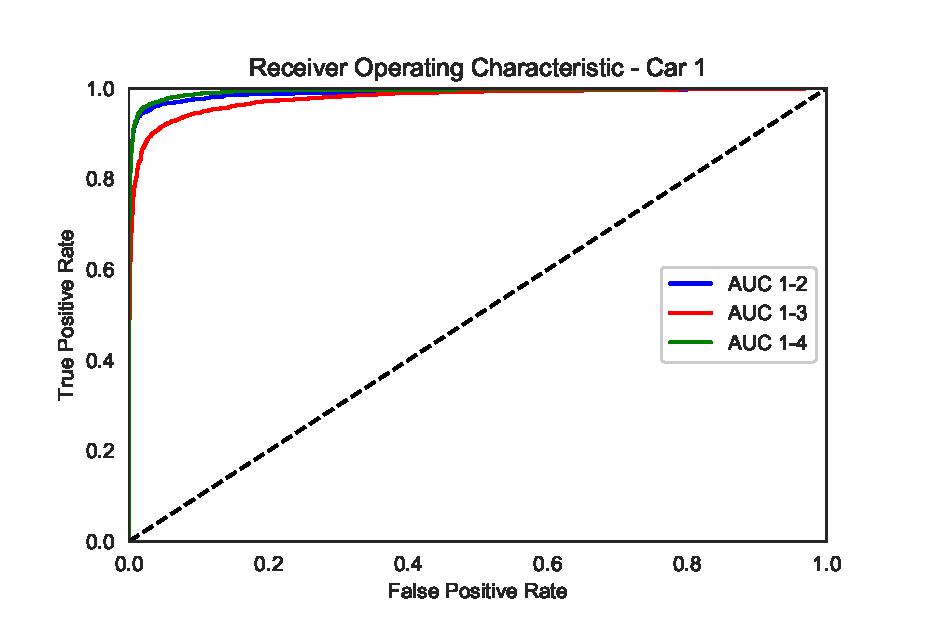
\includegraphics[width=0.4\textwidth]{auc12.eps}} 
    \subfigure[Veículo 2]{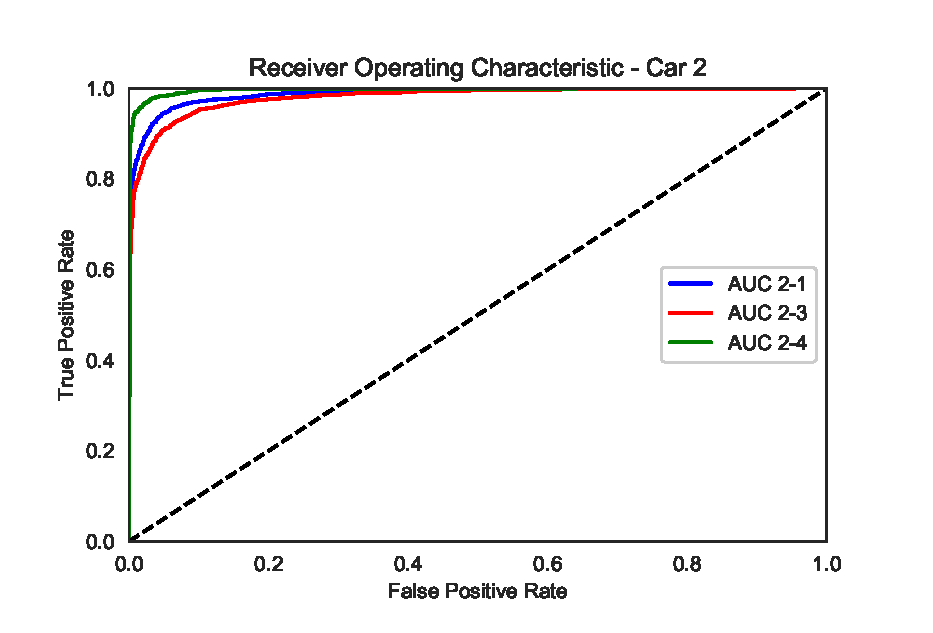
\includegraphics[width=0.4\textwidth]{auc22.eps}}}
\makebox[\linewidth][c]{
    \subfigure[Veículo 3]{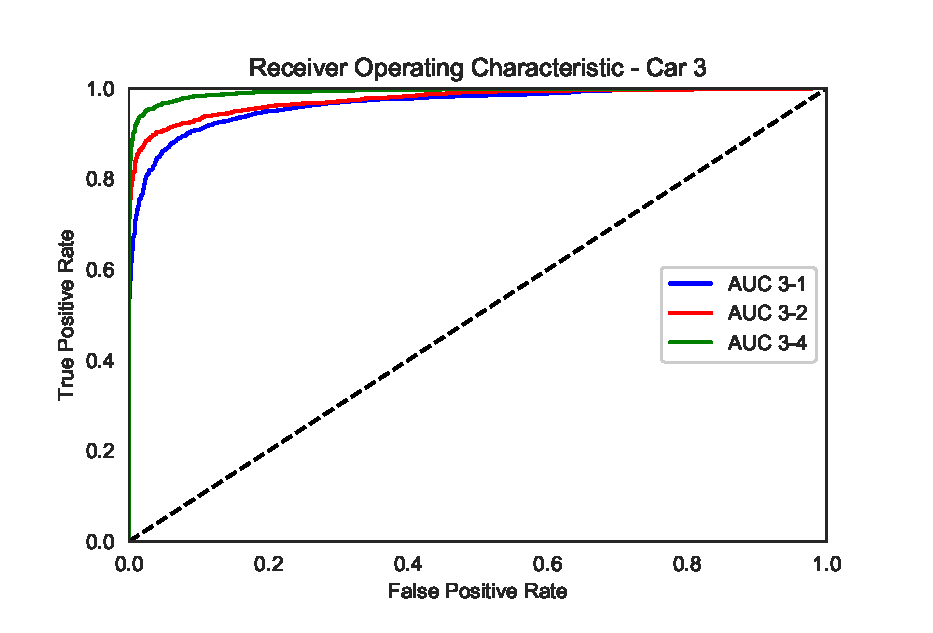
\includegraphics[width=0.4\textwidth]{auc32.eps}}
    \subfigure[Veículo 4]{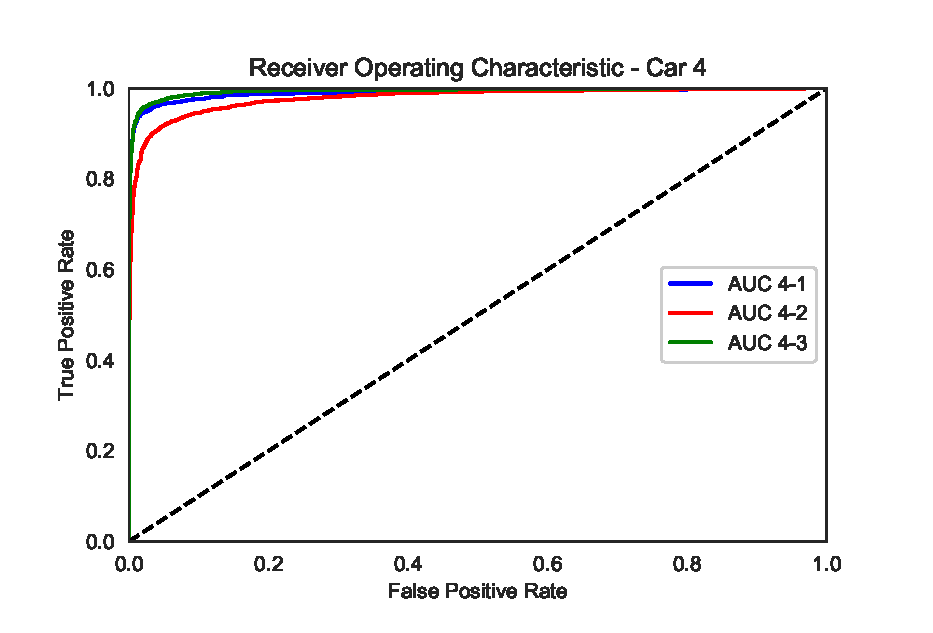
\includegraphics[width=0.4\textwidth]{auc42.eps}}}
    \caption{Curva ROC para cada um dos veículos.}
    \label{fig:roc}
\end{figure*}

\section{Considerações Finais} \label{sec:finais}

O presente trabalho teve como objetivo apresentar, até onde se sabe, a inédita aplicação de redes neurais siamesas como codificador não linear de dados de direção para a implementação de um sistema de autenticação de condutores que não demande de ser retreinando a cada novo veículo que empregue o sistema e a cada novo condutor autorizado para este veículo. Esta codificação funciona como um extrator de características que transforma o conjunto de dados de entrada de cada condutor em uma representação aglomerada espacialmente para amostras de um mesmo condutor e espaçadas de dados outros condutores.

Esta representação espacial gerada pela rede base da RNS foi usada para gerar a representação espacial de outros condutores que não foram utilizados no treinamento da RNS, de modo a gerar um suporte de dados de cada um deles. Este suporte é usado pelo algoritmo NN, baseado em distância, que não demanda de treinamento. Se a menor distância entre a amostra de um condutor desconhecido e o ponto no suporte mais próximo a esta amostra for menor que o um limiar determinado este condutor é considerado autêntico. Os resultados obtidos indicam que o modelo de autenticação de condutores consegue discernir com sucesso entre condutores autorizados e impostores a uma AUC superior a 99\%, para um grupo de condutores que não estiveram presentes no treinamento da rede neural siamesa.

Uma das limitações para determinar a real eficiência do modelo é que o \textit{dataset} utilizado possui apenas uma seção de direção de cada condutor. Sem a disponibilidade de diferentes seções, não é possível analisar se o modelo consegue aproximar dados de um mesmo condutor em diferentes circunstâncias. Em trabalhos futuros espera-se a obtenção e uso de dados com maior variabilidade de situações, o que traria ao modelo RNS uma maior robustez. Contudo, os resultados apresentados indicam a viabilidade da aplicação de RNS para o problema de autenticação de condutores.

% BIBLIOGRAFIA
\bibliography{exemplo}
\end{document}
